\documentclass[a4paper, 12pt]{article}

\usepackage[portuges]{babel}
\usepackage[utf8]{inputenc}
\usepackage{amsmath}
\usepackage{indentfirst}
\usepackage{graphicx}
\usepackage[colorinlistoftodos]{todonotes}
\usepackage{listings}
\graphicspath{{images/}}
\usepackage{xcolor}
\usepackage{float}
\usepackage{wrapfig}

\definecolor{codegreen}{rgb}{0,0.6,0}
\definecolor{codegray}{rgb}{0.5,0.5,0.5}
\definecolor{codepurple}{rgb}{0.58,0,0.82}
\definecolor{backcolour}{rgb}{0.95,0.95,0.92}

\lstdefinestyle{mystyle}{
    backgroundcolor=\color{backcolour},   
    commentstyle=\color{codegreen},
    keywordstyle=\color{magenta},
    numberstyle=\tiny\color{codegray},
    stringstyle=\color{codepurple},
    basicstyle=\ttfamily\footnotesize,
    breakatwhitespace=false,         
    breaklines=true,                 
    captionpos=b,                    
    keepspaces=true,                 
    numbers=left,                    
    numbersep=5pt,                  
    showspaces=false,                
    showstringspaces=false,
    showtabs=false,                  
    tabsize=2
}

\lstset{style=mystyle}
\usepackage{hyperref}
\hypersetup{
    colorlinks=true,
    linkcolor=blue,
    filecolor=magenta,      
    urlcolor=cyan,
    pdftitle={Overleaf Example},
    pdfpagemode=FullScreen,
    }

\urlstyle{same}


\begin{document}
%\maketitle

\begin{titlepage}
	\begin{center}
		\huge{Universidade Federal do Rio de Janeiro}

\vspace{10pt}
\begin{figure}[!ht]
\centering

\includegraphics[width=3cm]{minerva.eps}
\hspace{3cm}

\includegraphics[height=3cm, width=7cm]{poli-logo.pdf}
\end{figure}
        
        \vspace{85pt}
        
		\textbf{\LARGE{Relatório de Laboratório}}
		\large{\\
        		Desenvolvimento de uma ULA}
		\vspace{160pt}
		
	\end{center}
	
	\begin{flushleft}
		\begin{tabbing}
			Alunos\qquad\qquad\= Pedro Henrique Grave Lima\\
			\>Marina Sangineto Jucá\\
            \> Arthur N Trucco\\
            \> Rodrigo Leal \\
            \> Luiz Felipe Cantanhede Cristino \\
			Professor\> Roberto Gonçalves Pacheco \\
			Horário\> Ter - 13:00-15:00\\
		
	\end{tabbing}
		  
	\end{flushleft}
	
	\begin{center}
		\vspace{\fill}
		Rio de Janeiro, \today
	\end{center}
\end{titlepage}
%%%%%%%%%%%%%%%%%%%%%%%%%%%%%%%%%%%%%%%%%%%%%%%%%%%%%%%%%%%
\newpage
\tableofcontents
\thispagestyle{empty}

\newpage
\pagenumbering{arabic}

%%%%%%%%%%%%%%%%%%%%%%%%%%%%%%%%%%%%%%%%%%%%%%%%%%%%%%%%%
%%%%%%%%%%%%%%%%%%%%%%%%%%%%%%%%%%%%%%%%%%%%%%%%%%%%
\section{Introdução}

Este documento tem como objetivo relatar o desenvolvimento do trabalho proposto. O trabalho constitui a construção de uma Unidade Lógica Aritmética (ULA) de quatro bits que seja capaz de realizar oito operações distintas. Dentre essas operações, quatro são obrigatórias, sendo elas as operações de soma, subtração em complemento de 2, incremento de +1 e troca sinal. Entre as não obrigatórias, optamos por realizar as operações de multiplicação, mod, potência de 2 e comparador.
\section{Desenvolvimento}

Para a realização deste trabalho foi-se desenvolvido e testado um código em linguagem de descrição de hardware (VHDL) no laboratório da disciplina, onde foram produzidos os resultados bases em uma placa FPGA. A partir desses resultados, o projeto continuou a ser desenvolvido de maneira remota através do uso de softwares e ferramentas de produção, como o Quartus Prime Lite, GitHub e Overleaf. 

\section{Operações Obrigatórias}


\subsection{Adição}


Para implementação da operação de adição, foi-se necessária a implementação, primeiramente, de um \textit{full adder} de 1 bit, para que, a partir dele, construir um \textit{full adder} de 4 bits.

\subsubsection{1 bit full adder}

\begin{lstlisting}[language=VHDL]
Y <= (A xor B) xor Cin;
Cout <= (A and B) or ((A xor B) and Cin);
\end{lstlisting}


\subsubsection{4 bit full adder}


\begin{lstlisting}[language=VHDL]
-- fa de 4 bits e composto de 4 fas de 1 bit
fa0: fa port map(x(0), y(0), C_in, c1, s(0));
fa1: fa port map(x(1), y(1), c1, c2, s(1));
fa2: fa port map(x(2), y(2), c2, c3, s(2));
fa3: fa port map(x(3), y(3), c3, c4, s(3));

Z <= s;
C_out <= c4;

Flags(3) <= '1' when S = "0000" else '0';       -- zero
Flags(2) <= not c4 and C_in;				        -- negativo
Flags(1) <= c4;	                                -- cout
Flags(0) <= c4 and (not C_in); 					    -- overflow
\end{lstlisting}

\subsection{Subtração em Complemento de 2}
Este módulo é constituído pela adição da primeira entrada Xs com o complemento de 2 da segunda entrada Ys.

\begin{lstlisting}[language=VHDL]
-- adicao de A + (-B) em complemento de dois
-- Adicionamos A + C2(B), fazendo o complemento com o not e Cin=1
A <= Xs;
B <= not Ys;

fulla : fourbitfa port map(A, B, '1', C_outs, Zs, Flagss);
\end{lstlisting}


\subsection{Incremento de +1}
Este módulo soma o bit +1 à entrada Xi.

\begin{lstlisting}[language=VHDL]
-- simples adicao do valor 1 ao valor de entrada X
ADD1: fourbitfa port map(Xi, "0001", '0', C_outi, Zi, Flagsi);
\end{lstlisting}

\subsection{Troca de Sinal}
A operação de troca de sinal é feita fazendo o complemento a dois do número em questão.
\begin{lstlisting}[language=VHDL]
-- Complemento a dois e feito com a inversao do numero e incremento +1
A <= not Xcpl;
B <= "0000";

ADD1:fourbitfa port map(A, B, '1', C_outcpl, Zcpl, Flagscpl);
\end{lstlisting}

\section{Operações Livres}

\subsection{Multiplicação}
A então operação de multiplicação foi implementada utilizando componentes ja implementados \textit{full adders} de 4 bits. Graças a limitação de LEDs na placa, a saída foi 'truncada' de forma que só mostra-se os quatro bits menos significantes, indicando \textit{overflow} caso o produto tenha mais que quatro bits.

\begin{lstlisting}[language=VHDL]
XY(0)<= Xm(0) and Ym(0);
XY(1)<= Xm(1) and Ym(0);
XY(2)<= Xm(2) and Ym(0);
XY(3)<= Xm(3) and Ym(0);

XY(4)<= Xm(0) and Ym(1);
XY(5)<= Xm(1) and Ym(1);
XY(6)<= Xm(2) and Ym(1);
XY(7)<= Xm(3) and Ym(1);

XY(8)<= Xm(0) and Ym(2);
XY(9)<= Xm(1) and Ym(2);
XY(10)<= Xm(2) and Ym(2);
XY(11)<= Xm(3) and Ym(2);

XY(12)<= Xm(0) and Ym(3);
XY(13)<= Xm(1) and Ym(3);
XY(14)<= Xm(2) and Ym(3);
XY(15)<= Xm(3) and Ym(3);

K0 <= (XY(7),XY(6),XY(5),XY(4));
K1 <= (XY(11),XY(10),XY(9),XY(8));
K2 <= (XY(15),XY(14),XY(13),XY(12));
conn0 <= ('0',XY(3),XY(2),XY(1));

P(0) <= XY(0);
	 
FBM1: fourbitfa port map ( X=>K0,Y=>conn0,C_in=>'0',
                                   C_out=>conn1(3),
                                   Z(3)=>conn1(2),Z(2)=>conn1(1)
											  ,Z(1)=>conn1(0),Z(0)=>P(1));
											
FBM2: fourbitfa port map ( X=>K1,Y=>conn1,C_in=>'0',
                                   C_out=>conn2(3),
                                   Z(3)=>conn2(2),Z(2)=>conn2(1)
											  ,Z(1)=>conn2(0),Z(0)=>P(2));
											  
FBM3: fourbitfa port map ( X=>K2,Y=>conn2,C_in=>'0',
                                   C_out=>P(7),
                                   Z => P(6 downto 3)
											  );
											  
Zm(0) <= P(0);
Zm(1) <= P(1);
Zm(2) <= P(2);
Zm(3) <= P(3);

-- conferindo overflow								
Flagsm(0) <= '1' when P > "00001111" else '0';

-- conferind zero
Flagsm(3) <= '1' when P = "00000000" else '0';

--cout
Flagsm(1) <= '0';

--negativo
Flagsm(2) <= Xm(3) xor Ym(3);
\end{lstlisting}

\subsection{AND}
Este módulo consiste na função lógica AND entre as duas entradas.
\begin{lstlisting}[language=VHDL]
Zand <= Xand and Yand;
\end{lstlisting}

\subsection{XOR}
Este módulo consiste na função lógica AND entre as duas entradas.
\begin{lstlisting}[language=VHDL]
Zxor <= Xxor xor Yxor;
\end{lstlisting}

\subsection{Comparador}
Neste módulo, realizou-se a implementação de uma função de comparação, de forma que o \textit{input} Xq é comparado com o \textit{input} Yq, e indica-se, na saída se o primeiro é maior, igual ou menor.

\begin{lstlisting}[language=VHDL]
process(Xq, Yq)
    begin
        if Xq > Yq then
            Greater <= '1';
            Equal   <= '0';
            Less    <= '0';
        elsif Xq = Yq then
            Greater <= '0';
            Equal   <= '1';
            Less    <= '0';
        else
            Greater <= '0';
            Equal   <= '0';
            Less    <= '1';
        end if;
    end process;
Zq(0) <= Less;
Zq(1) <= Equal;
Zq(2) <= Greater;
\end{lstlisting}


\section{Troca de Operações e Entradas}
A fim de permitir que as operações sejam alterados para a execução de todas as funcionalidades presentes na ULA, foi proposto o desenvolvimento e aplicação do seguinte bloco de código:
\begin{lstlisting}[language=VHDL]
process (CLOCK_50) is
   begin
		case op is
		-- verifica qual operacao esta sendo selecionada
			when "000" => 
			--soma
				Zop <= add_out;
				Flg <= add_flags;

			when "001" =>
			--complemento 2
				 Zop <= comp_out;
				 Flg <= comp_flags;

			when "010" =>
			--subtrao
				 Zop <= sub_out;
				 Flg <= sub_flags;

			when "011" =>
			--incremento +1
				Zop <= inc_out;
				Flg <= inc_flags;
			----------------------------------------
			when "100" =>
			--comparador
				Zop <= qual_out;
				Flg <= "0000";

			when "101" =>
			--and
				Zop <= and_out;
				Flg <= "0000";

			when "110" =>
			--xor
				Zop <= xor_out;
				Flg <= "0000";

			when "111" =>
			--multiplicacao
				Zop <= mult_out;
				Flg <= mult_flags;
			--------------------------------------------
			when others =>
			--caso de erro
				Zop <= "0000";
				Flg <= "0000";
        end case;
    end process;
\end{lstlisting}

Onde temos a seguinte tabela para definir o código de cada operação:

\begin{table}[htb]
\centering
\begin{tabular}{c|c}
Código & Operação \\ \hline
000	& Soma 		\\\hline
001 & Subtração	\\\hline
010 & Incremento \\\hline
011 & Sinal \\\hline
100 & Multiplicação \\\hline
101 & AND \\\hline
110 & XOR \\\hline
%101 & Mod \\\hline
%110 & Potência 2 \\\hline
111 & Comparador
\end{tabular}
\label{vazio}
\end{table}

\section{Resultados e Flags}

Simulando a ULA com o código modificado para uma resposta mais facilmente simulável (contador acelerado) obtemos o seguinte gráfico, onde é possível visualizar a saída de cada um dos módulos para um determinado instante de tempo.
\begin{figure}[H]
    \centering
    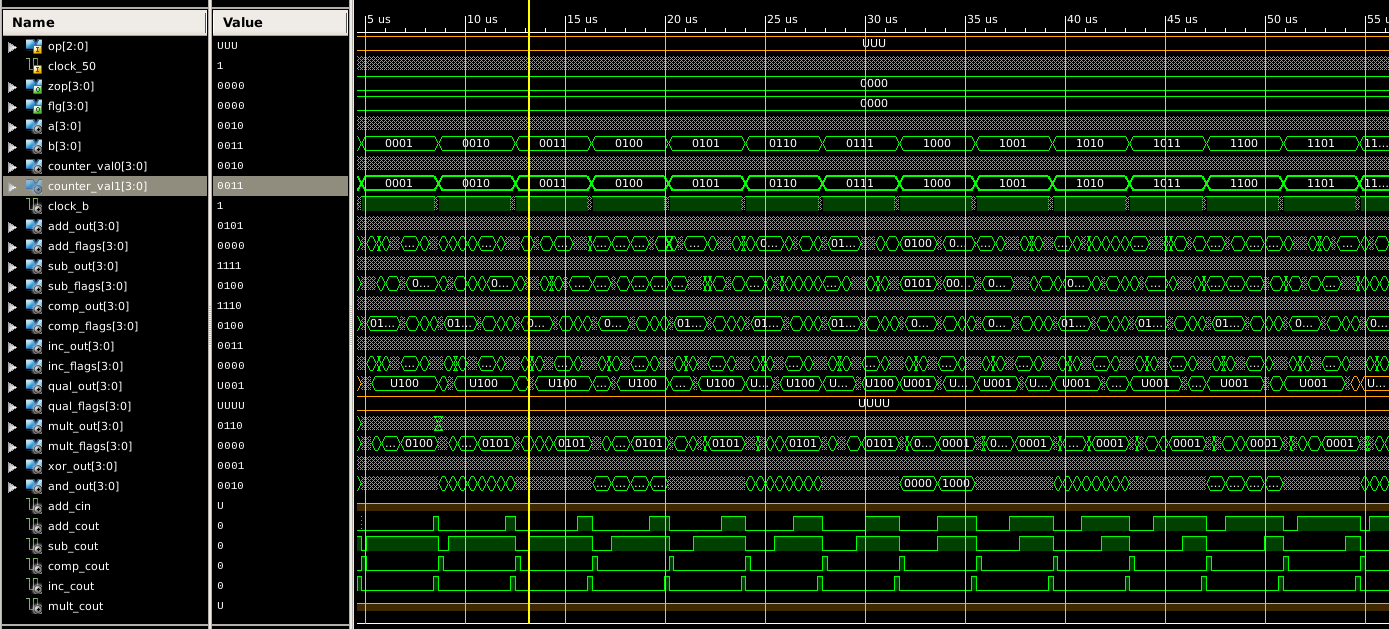
\includegraphics[width=13cm]{imagens/simu_sem_zoom.png}
    \caption{Resultados de simulação}
    \label{fig:simu}
\end{figure}
\begin{figure}[H]
    \centering
    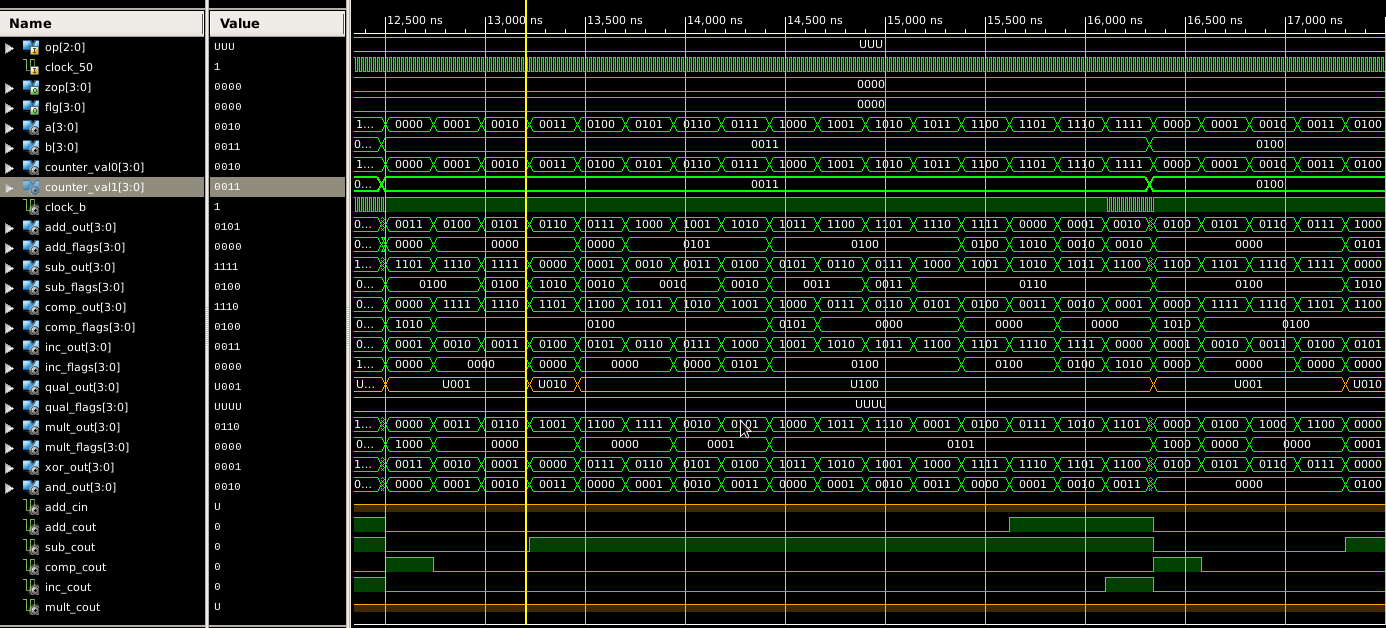
\includegraphics[width=13cm]{imagens/simu_com_zoom.png}
    \caption{Zoom mostrando a variação do contador que define o valor de A}
    \label{fig:simu_zoom}
\end{figure}

É válido notar que no resultado de cada operação também está presente os valores de todas as flags requisitados para plena compreensão do resultado: Zero, negativo, carry out e overflow.

\section{Conclusão}

Portanto, apesar das dificuldades enfrentadas na implementação das funções na placa, é possível concluir que a construção teórica desenvolvida ao longo dos laboratórios fundamentou um código o qual é capaz de simular perfeitamente uma ULA. Os resultados obtidos foram os esperados e, por fim, é possível destacar que o objetivo do trabalho prático foi alcançado.


\end{document}